\documentclass{article}
\usepackage[utf8]{inputenc}

% All of the setup stuff that used to go here I've shoved into foar705journal.sty since that's much better practice than copy-pasta
\usepackage{foar705journal}

%https://en.wikibooks.org/wiki/LaTeX/Modular_Documents#Separate_compilation_of_child_documents
\usepackage{subfiles}


%https://www.overleaf.com/learn/latex/Code_Highlighting_with_minted
%http://tug.ctan.org/macros/latex/contrib/minted/minted.pdf
\usepackage{minted}

\usepackage{graphicx}
\graphicspath{{./Figures/}}


\usepackage{enumitem}
%https://tex.stackexchange.com/a/447322

\newcommand{\startdeflist}[0]{%
\begin{description}[style=unboxed, labelwidth=\linewidth, font =\sffamily\itshape\bfseries, listparindent =0pt, before =\sffamily]}

\title{Learning Journal Weeks 9 - 13}
\author{Bree Kelly}
\date{}


\begin{document}

\maketitle
%this needs to be inside the document because LaTeX

\tablesofcontentsanderrors

\section{Tuesday October 15th 2019}

\section{Data Carpentry}
\textbf{Intention} Complete Data Carpentry on R, lessons 3 and 4.

\textbf{Actions} Following the instructions on the Data Carpentry website, I go through the lessons and answer the following questions:

\subsection{Lesson 3: Starting with Data}

\subsubsection{What is a data.frame?}

The representation of data in the format of a table where the columns are vectors that all have the same length. It is a data structure that forms a building template for data. It does the same thing every time. Infrastructure for data.

\textit{How can I read a complete csv file into R?}

Run the function \mintinline{R}|read_csv(filename)|. 

You can also use the function view to see it in the top left pane.

\textit{How can I get basic summary information about my dataset?}

Using functions such as dim() (no. of rows and columns), nrow() (no. of rows), ncol() (no. of columns), head() (shows first 6 rows), tail() (shows last 6 rows), names() (shows column names), str() (structure of object), and finally summary() (returns summarised statistics for each column).

\textit{How do I convert between strings and factors?}

Using factor()

\textit{Describe the difference between a factor and a string.}

I'm not sure about this one.

\textit{Why would I want strings to be treated differently?}

Depends on the type of data analysis you wish to employ and how you what to extract information.

\textit{How do I reorder and rename factors?}

By specifying the factor you wish to rename using [] with an integer inside and assigning (using an arrow) the new name. To reorder them, you use the assign function, combine function and factor function, eg.
\begin{minted}[breaklines]{R}
memb_assoc <- factor(memb_assoc, levels = c("No", "Yes", "Undetermined"))
\end{minted}
\textit{How do I change how character strings are handled in a data frame?}

Turn them into numerical integers, eg, `as.numeric(as.character(year\_fct))'

\itemizederror{No package called `Tidyverse'}{
\item I started by downloading R and RStudio onto my laptop, then switching to my Surface, on which the CSV file of cleaned SAFI data that I produced in the OpenRefine Data Carpentry Lessons is located. I followed the instructions to download tidyverse in order to use the read\_csv() function, but running library(tidyverse) returned `Error in library(tidyverse) : there is no package called ``tidyverse'' I swear I already downloaded that package, but okay. I go to the Packages tab and search `tidy.' No tidyverse package. I click Install and select tidyverse and set it installing. Installation is a success.}

I run library(tidyverse) again. It returns this:

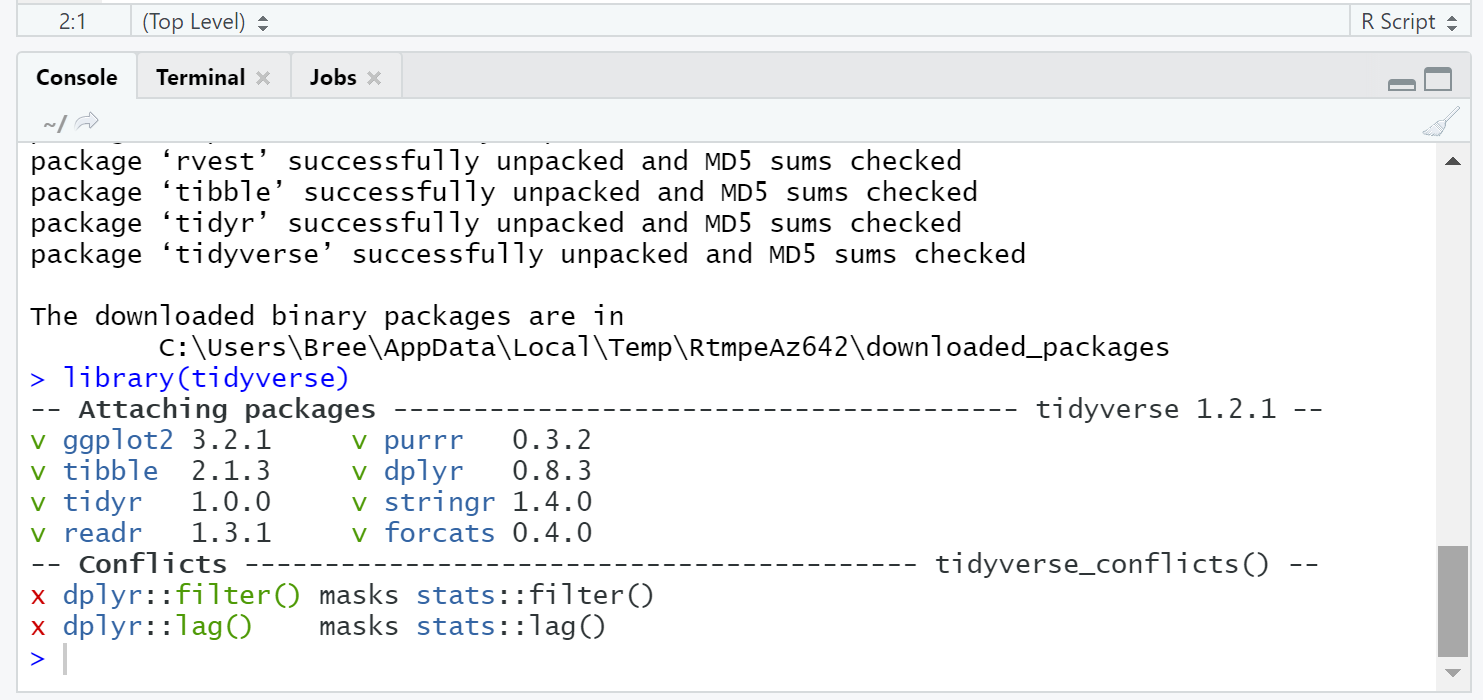
\includegraphics[width=1.0\textwidth]{rstudio_14.PNG}

I copy the CSV file I want to work with (``SAFI\_clean\_exercise\_CSV.csv") into the working directory (Computer/Documents/). I run 

\begin{verbatim}
    interviews <- read_csv("SAFI_clean.csv", na = "NULL") 
\end{verbatim}

 as per the instructions, leaving out the part of the file name I added (ie. `\_exercise\_CSV') because I am an idiot. Of course, this is returned: ``Error: unexpected `NULL' in 
 
 ``interviews \<\- read\_cscv(``SAFI\_clean.csv, na = ``NULL")" I now notice I left out the double quotation mark at the end of the file name, so I correct this, and it finally prints the following:

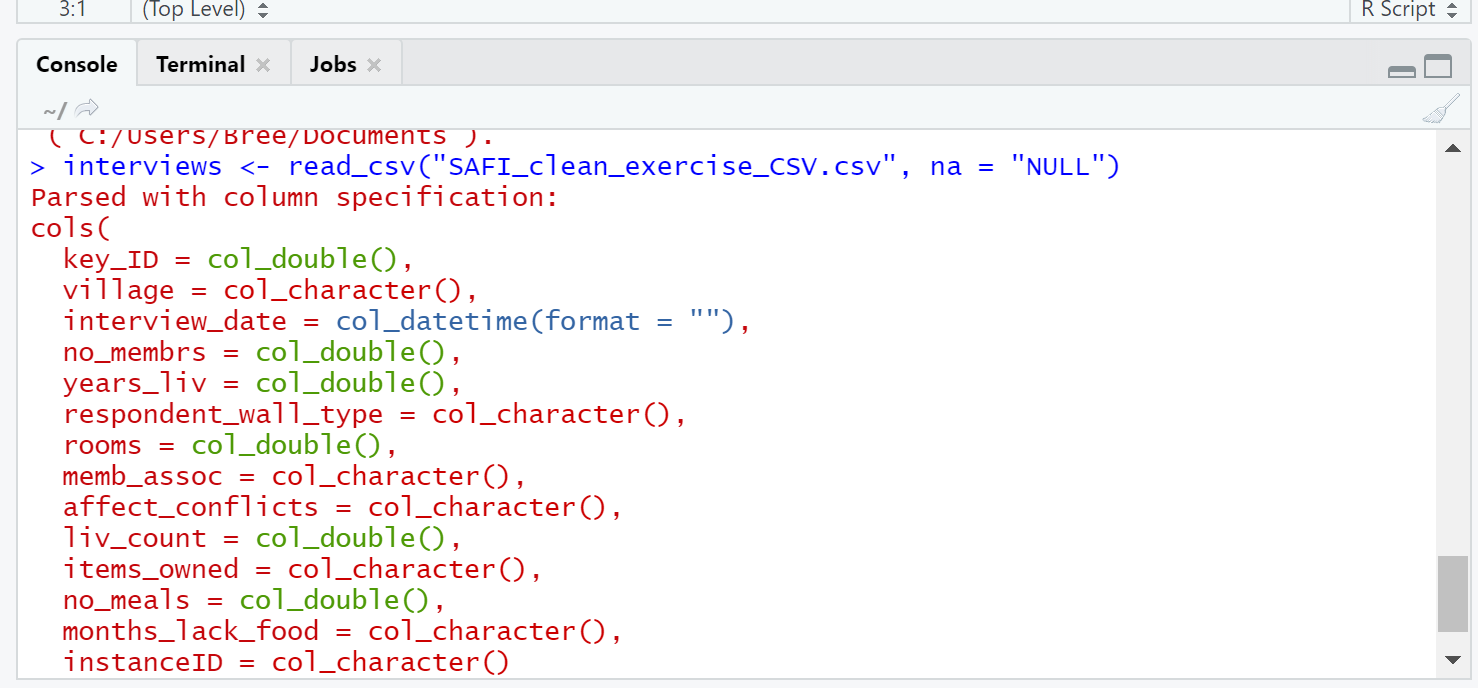
\includegraphics[width=1.0\textwidth]{rstudio_15.PNG}

I can finally move on. I try running just `interviews' to see the file:

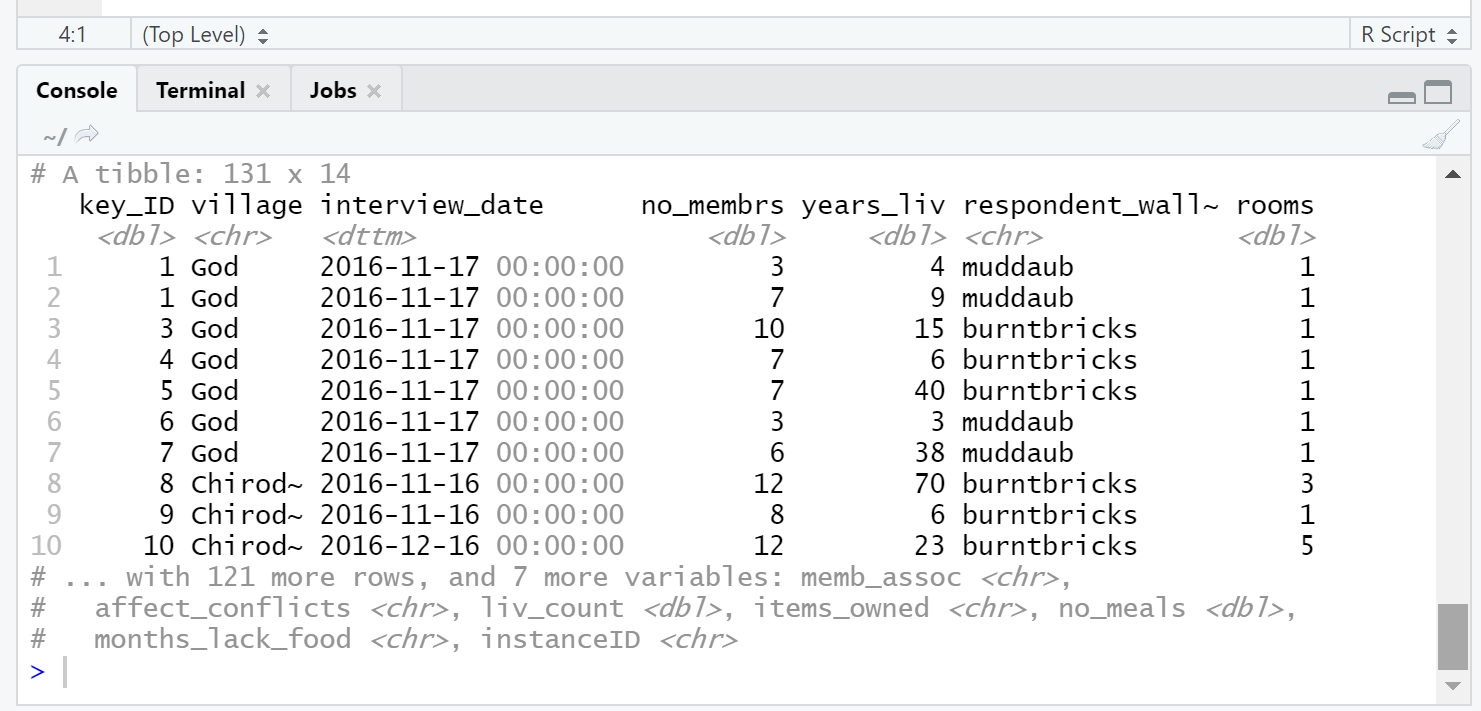
\includegraphics[width=1.0\textwidth]{rstudio_16.PNG}

I then try `view(interviews),' which returns an excel-sheet-looking table in a new tab within the top left pane:

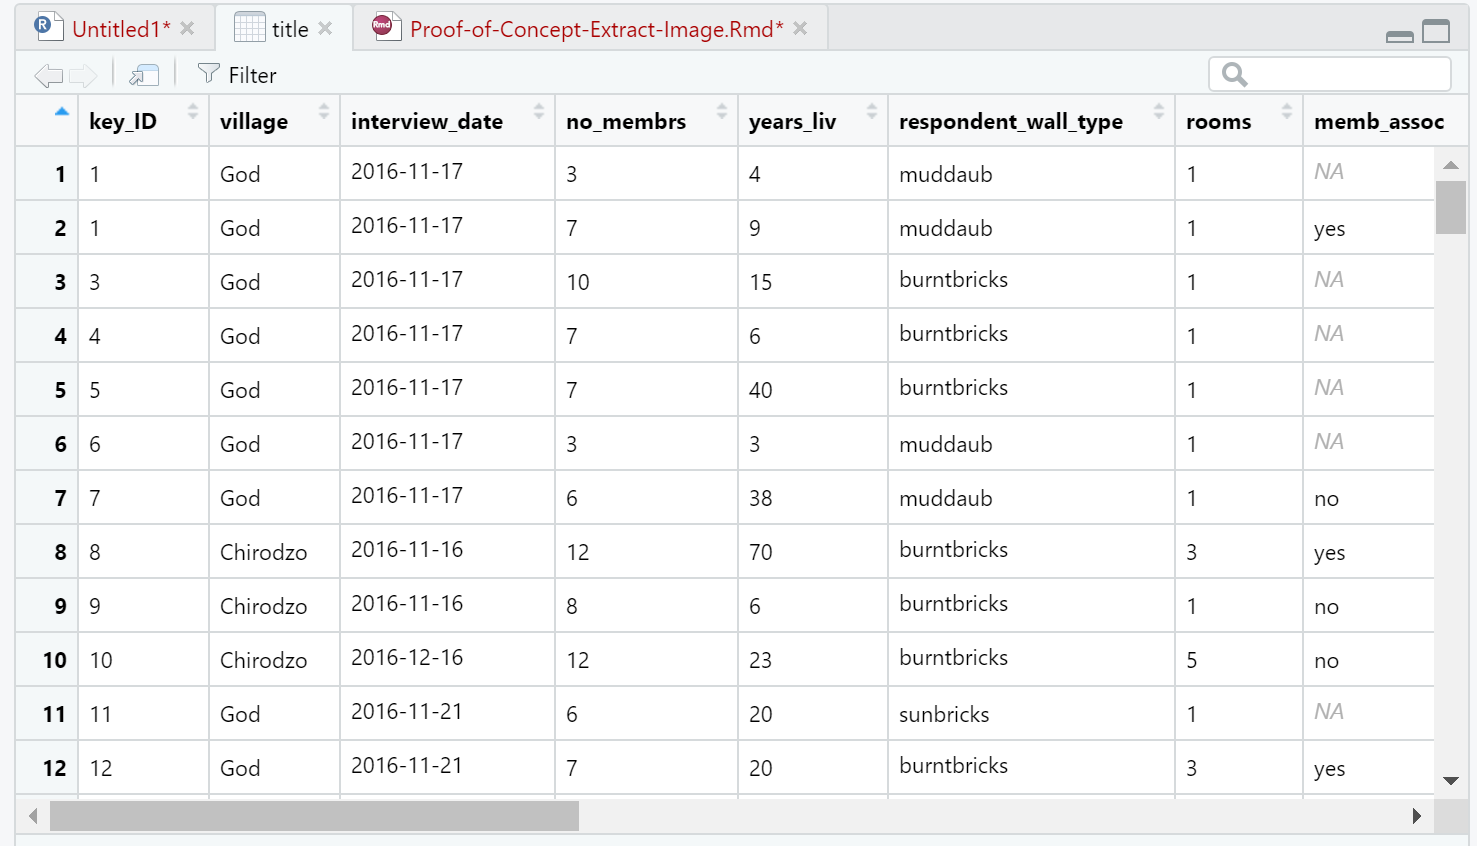
\includegraphics[width=1.0\textwidth]{rstudio_17.PNG}

I then try `head(interviews),' which returns this:

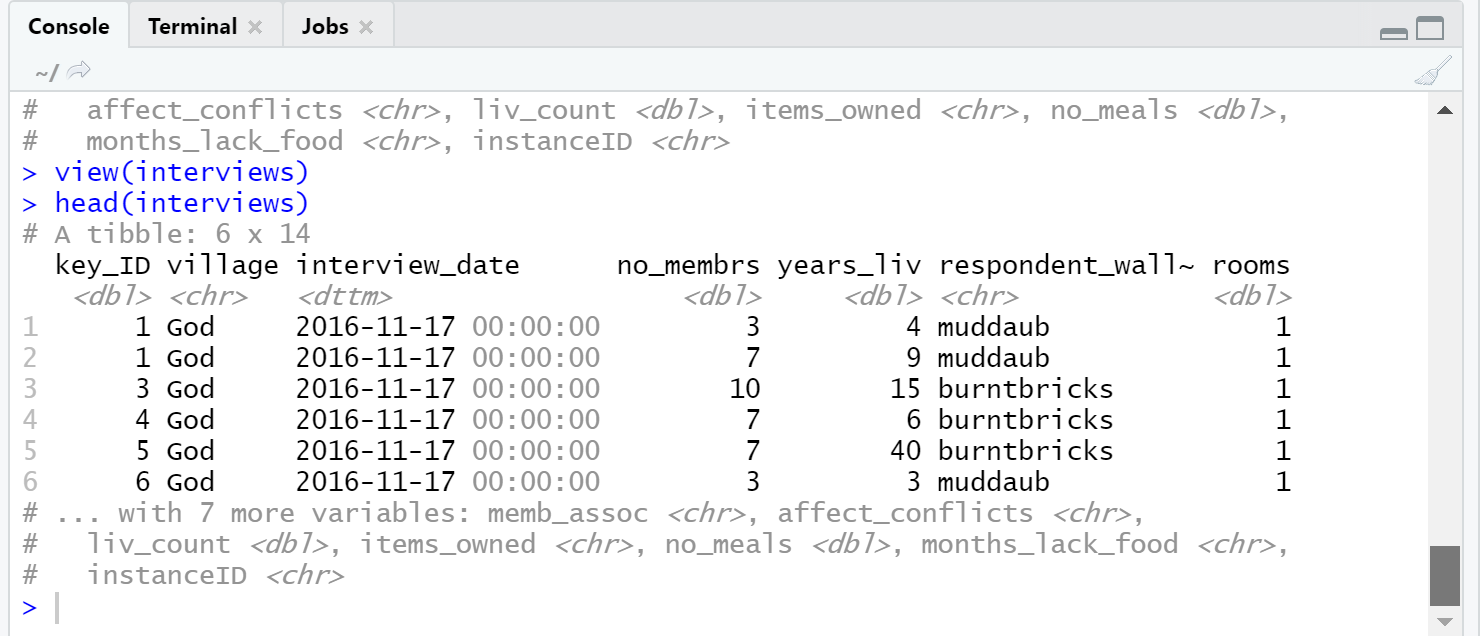
\includegraphics[width=1.0\textwidth]{rstudio_18.PNG}

Not sure how to interpret it, but I didn't get an error for once. I read further into the lesson that head(interviews) prints the first 6 lines of the file, which appears to be the case when I ran it. I run the various ways to specify columns and rows and such, including interviews[1, 1], interviews[1, 6] , interviews[[1]], interviews[1], interviews[1:3, 7], and interviews[3, ]. They all run fine, except with the last one, although it executes fine, I can see one difference in the results – instead of `8 more variables,' mine states that there are `7 more variables,' and appears to be missing the `rooms <dbl>.' I can also see a 1 after `burntbricks' on my console, which does not appear in the example. Maybe rooms is over there somewhere. I can't figure it out.

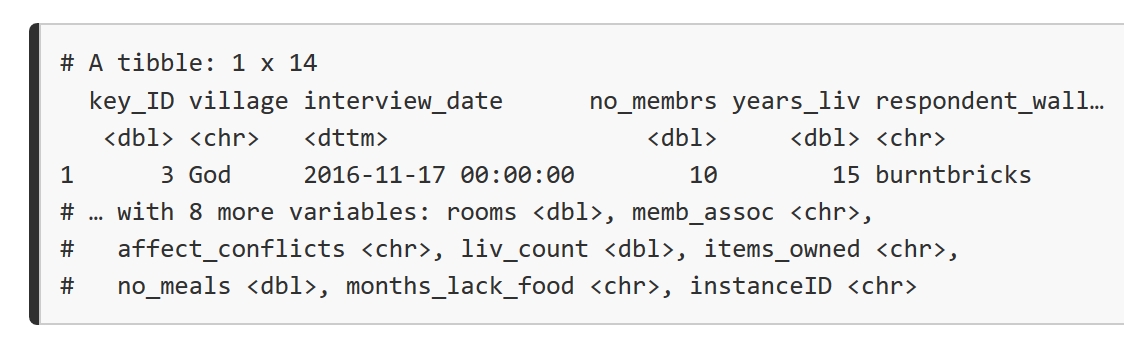
\includegraphics[width=1.0\textwidth]{rstudio_19.PNG}

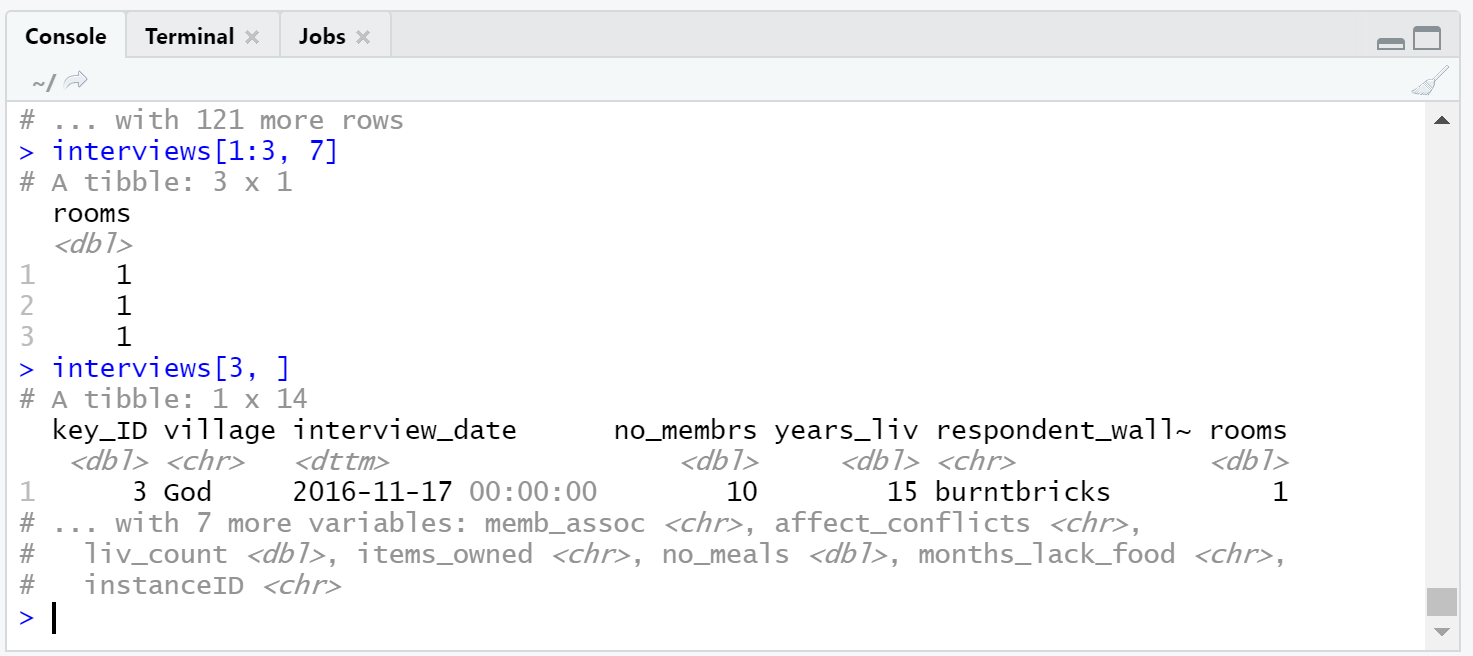
\includegraphics[width=1.0\textwidth]{rstudio_20.PNG}

I tried to complete the following exercise:

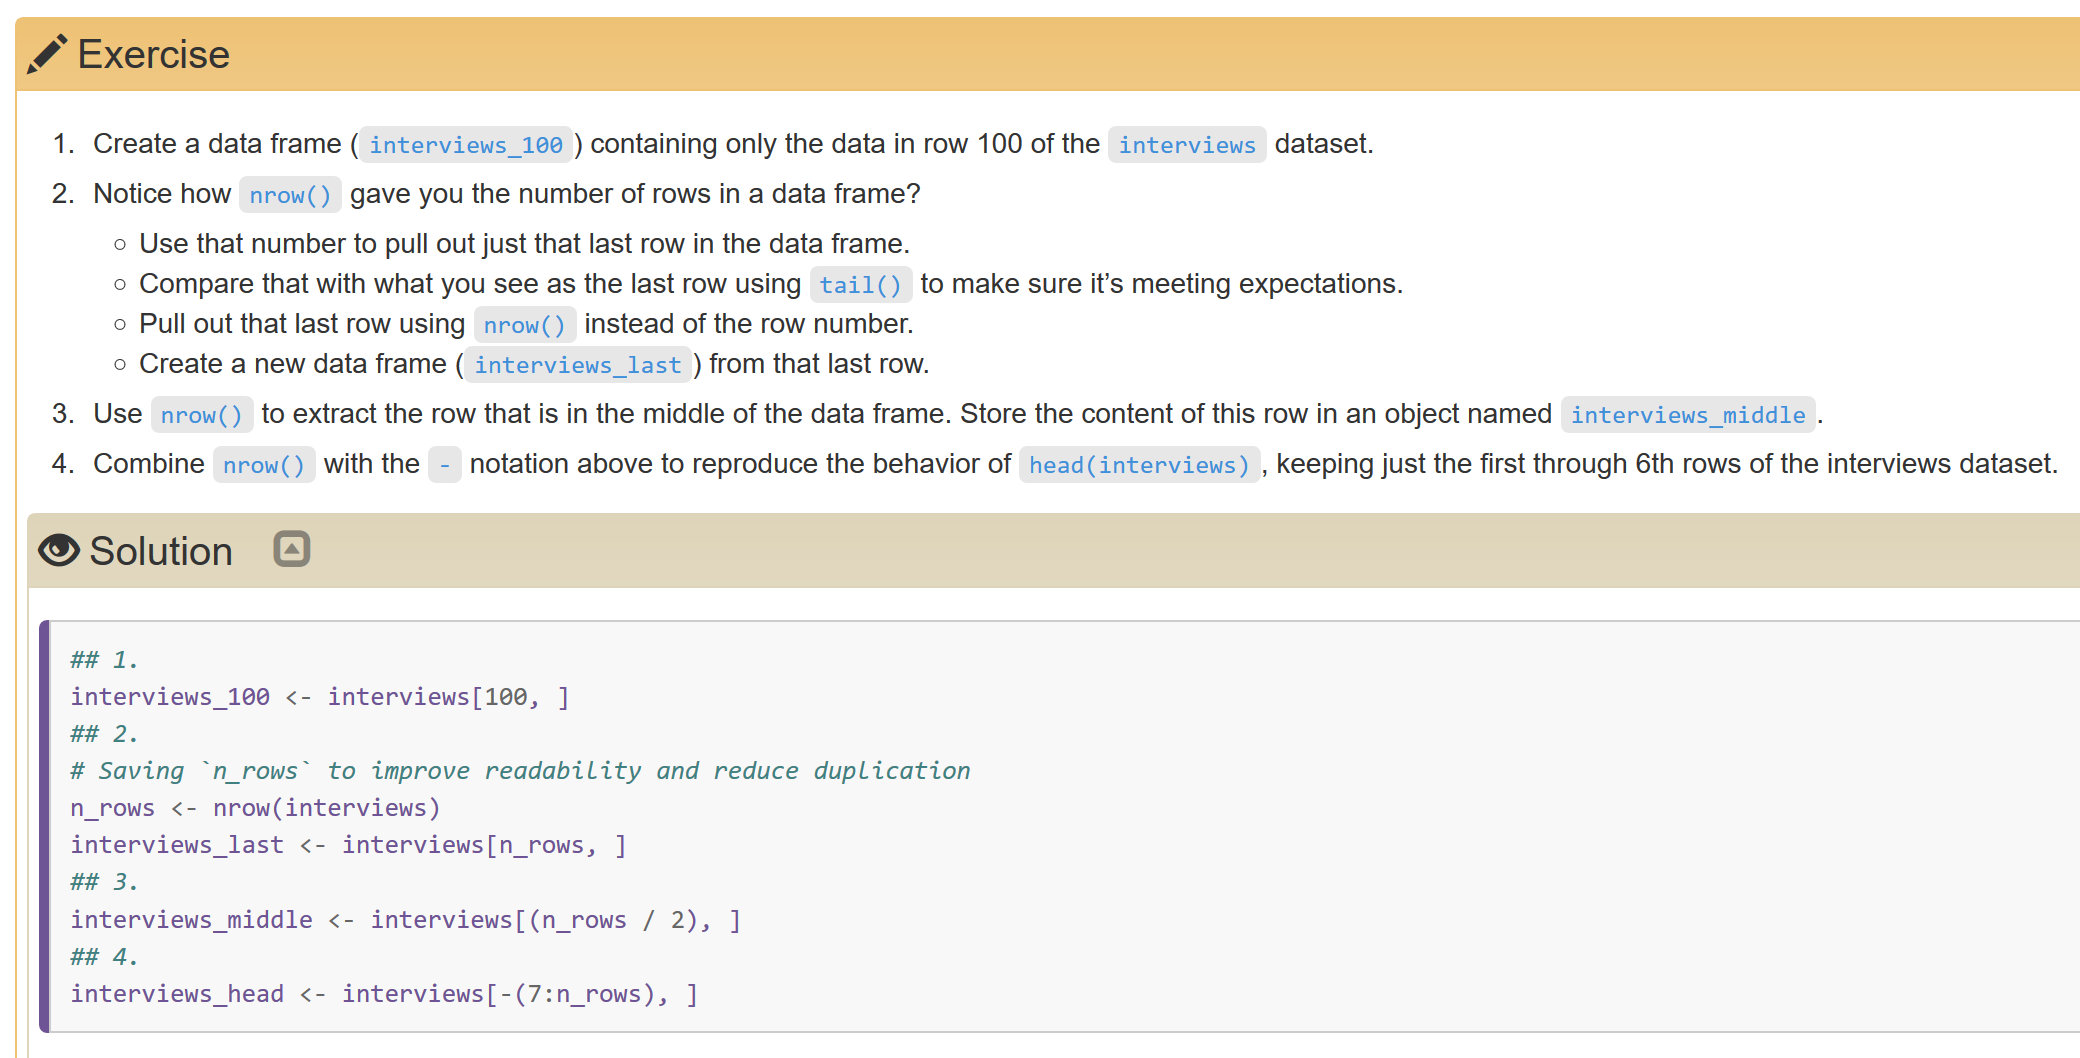
\includegraphics[width=1.0\textwidth]{rstudio_21.PNG}

I did the first part correctly (interviews \<\- interviews[100, ]), but got stuck after that. I feel like the instructions are not clear. The second part sounds like its using what you created in the first part, but that's not the case. I tried a few different things, but had to look at the Solution, and even then, I can't fully grasp what is happening in the exercise. I need more help and explanation on this one. Going through the lesson a second time, I think I understand it a little better, but I'm still not 100 on vector, strings, and factors.
\textbf{Result} Lesson 3 complete and recorded in Learning Journal.

\itemizederror{%Title of Error
Talking to Brian
}{% Itemized list of working through
\item Again rejected tea
\item Talked about job prospects
\item help?
}
% Much cleaner. 
% \tablesofcontentsanderrors

% \section{Stuff in the primary document, demonstrating foar705journal class}



% \lipsum[1]
% \subsection{Test subsection}
% \lipsum[1]
% \subsubsection{Test subsubsection}
% \lipsum[1]
% \subsection{Specific activity 1}
% \lipsum[1]
% \itemizederror{Test error via macro}{% 
% \item \lipsum[1]
% \item \lipsum[1]
% }

% \solution{%Explanation
% \lipsum[1]
% }{%Intention
% \lipsum[1]
% }{%Action
% \lipsum[1]
% }{%Result
% \lipsum[1]
% }


% \subsection{Error 1}
% \label{Error: This was a silly error}
% \lipsum[1]
% \subsection{Specific activity 1}
% \lipsum[1]
% \subsection{Non-displayed Error 2}
% \label{This was a different silly error that isn't displayed}
% \lipsum[1]
% \subsection{Displayed Error 3}
% \label{Error: This was a different silly error that is displayed}
% \lipsum[1-3]

% \itemizederror{Shell: A Whoopsiedoodle Functionality}{%
% \item Thing does not do thing
% \item When I try to undo, thing does not undo
% }

% \solution{It seems thing DOES do thing and I didn't realise thing was done.}
% {I will try Ctrl-C to cancel}
% {\texttt{$\wedge$C}}
% {I have done a learn.}

% \section{Importing subfiles}

% \subfile{Journals/subfile1.tex}
% \subfile{Journals/subfile2.tex}

\end{document}
